


\section{Test Area: The Rondonia State}
\par
The test area chosen for this thesis is the Amazon Rainforest, focusing specifically in the Rondonia state area. Rondonia topography is composed mainly by flat lands, which also have a lot of rivers thoroughout them, but also has regions of plateau with low altitude. The climate in Rondonia is what is called "humid equatorial" climate, which means that the temperature variation thorough the year is very little, something positive, since it is preferable to have no variations in the scene between SAR acquisition. The pluviometric indexes in the state can reach up to 2100mm per year, with most of the rains happening between May and September. The vegetation in the state (the focus of this thesis), just like most of north of Brazil, is the Amazon Rainforest, even though in some areas the \textit{Cerrado} vegetation is more common. The \textit{Cerrado} area is known for a very humid season and a very dry season, when the trees lose their leaves as a form of adaptation.
\par
The goal of this thesis is to improve algorithms to identify deforestation areas using SAR images. Because of that the natural choice of area to study was the Rondonia state, since it is the state with the most deforestation in the Amazon Rainforest. The Rondonia state already lost over 31\% of its forests and most of the remaining areas are degraded. For comparison, Acre, the state which borders Rondonia on the west, has 91\% of its original forest cover and a greater part of it is still intact. 
\par
Even though there are a lot of efforts being made to control the illegal deforestation, the results are not yet satisfactory and recent data even shows that the pace of deforestation have increased in the years of 2018 and 2019.\par
The deforestation in the Rondonia state can be easily seen with optical satellite data acquired with Google Earth. Deforestation follows a fairly predictable pattern, as seen in \figref{fig:fishbone}. The pattern of deforestation is known as fishbone pattern due to its similarity with a fish skeleton. This pattern arises from the fact that deforesting is normally done by penetrating the forest and then deforesting along the edges of the road firstly created.

\begin{figure}[H]
    \centering
    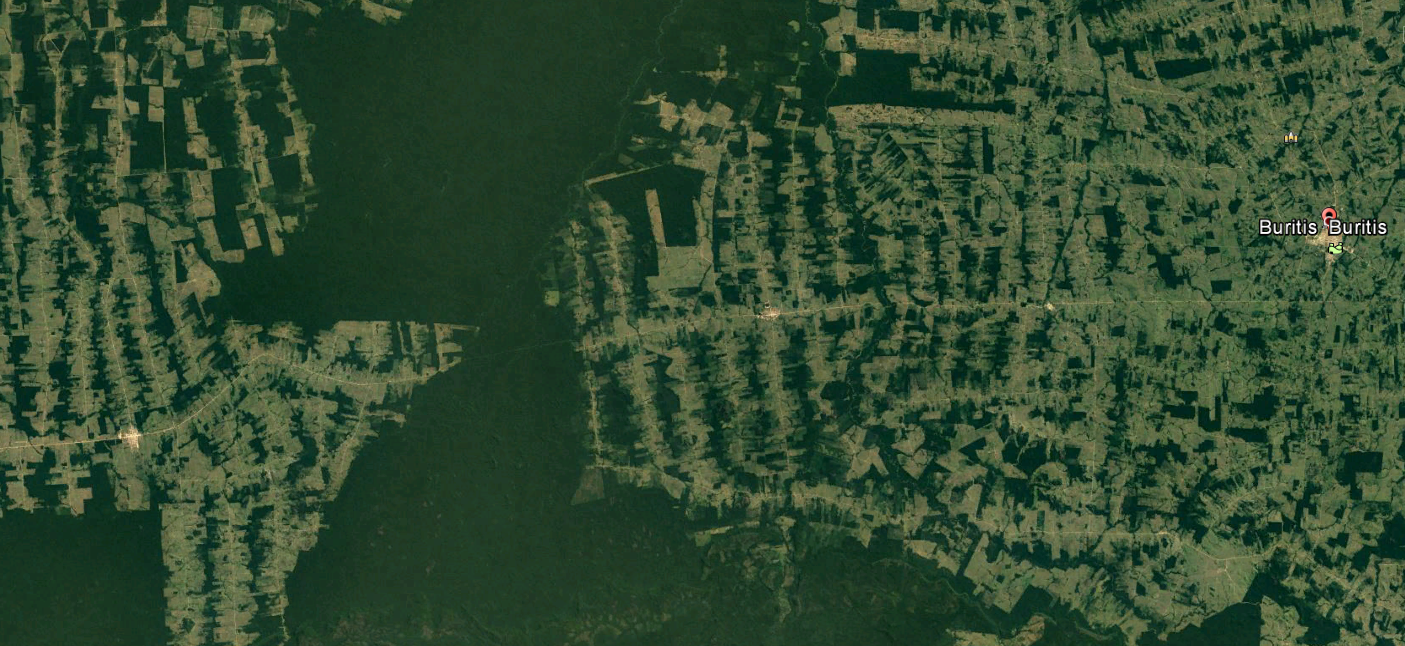
\includegraphics[width=0.8\linewidth]{Chapter2-real/fishbone.png}
    \caption{Fishbone pattern of deforestation.}
    \label{fig:fishbone}
\end{figure}{}

Due to recent fires that happened in the year of 2019 in the Amazon Rainforest, there is much concern about studying and monitoring the deforestation that happens in that area, and considering that the Rondonia state is the area in which the deforestation is most critical, it was a natural choice of area to study for this thesis. 

\section{TanDEM-X datasets}
TerraSAR-X (TSX) and TanDEM-X (TDX), launched in June 2007 and June 2010, respectively, are two German SAR satellites operating in X-band, developed within a public/private partnership
between the German Aerospace Center (DLR) and Airbus Defence and Space. 


The goal of both satellites is to provide SAR products for commercial purposes and scientific purposes, and the TanDEM-X mission has the primary goal of generatin a global, high precision, and consistent digital elevation model (DEM) with full coverage and no gaps. The relevance of the mission lies in that, until now, the available DEMs
of large parts of Earth are of low resolution, inconsistent, incomplete and commonly
based on different data sources and survey methods.\newline TanDEM-X has offered, for the first
time, a global, high accuracy and homogeneous DEM. Besides the main goal, other secondary missions based on along-track interferometry have been defined as well
as new techniques with bistatic SAR \cite{vintetres, vintequatro}. The work presented on this thesis is one of the possible exploitation of the activities of the TanDEM-X data.

\begin{figure}[H]
    \centering
    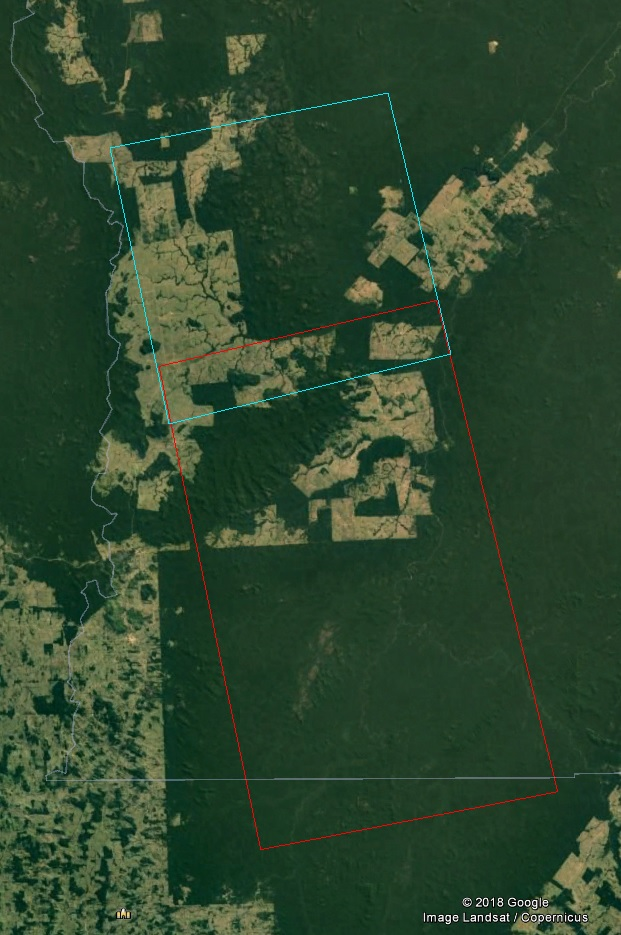
\includegraphics[width=0.6\linewidth]{Chapter2-real/tandem_dataset.jpg}
    \caption{TanDEM-X dataset available in Rondonia Area}
    \label{fig:tandem_dataset}
\end{figure}{}
TanDEM-X has the advantage that it can provide very high resolution data (each pixel has dimensions of  1.5m X 1.5m). Since the data is very resolution, and therefore very big in terms of memory size, it was chosen to work with small areas in the Rondonia state.
The dataset available is on the east of the Rondonia State. It was collected images from two areas in east Rondonia as can be seen in \figref{fig:tandem_dataset}. Each rectangle represents one SAR image acquired with the TanDEM-X.

\section{Sentinel-1 datasets}
\par
The SENTINEL-1 mission is a joint initiative of the European Commission (EC) and the European Space Agency (ESA). Copernicus, previously known as GMES, is a European initiative for the implementation of information services dealing with environment and security. It is based on observation data received from Earth Observation satellites and ground-based information.

Sentinel-1 is an imaging radar mission operating in C-band consisting of a constellation of two satellites aimed at providing day and night supply of imagery for users, independent of the weather at the time.
It also provides dual polarisation capability, very short revisit times and rapid product delivery. 
The constellation of two satellites, SENTINEL-1A and SENTINEL-1B, shares the same orbital plane.
\par
According to \cite{sentinelmission} there are five priorities for the SENTINEL-1 mission: To monitor sea ice zones and the arctic environment, surveillance of marine environment, to monitor land surface motion risks, mapping of land surfaces and mapping in support of humanitarian aid in crisis situations.

\begin{figure}[H]
    \centering
    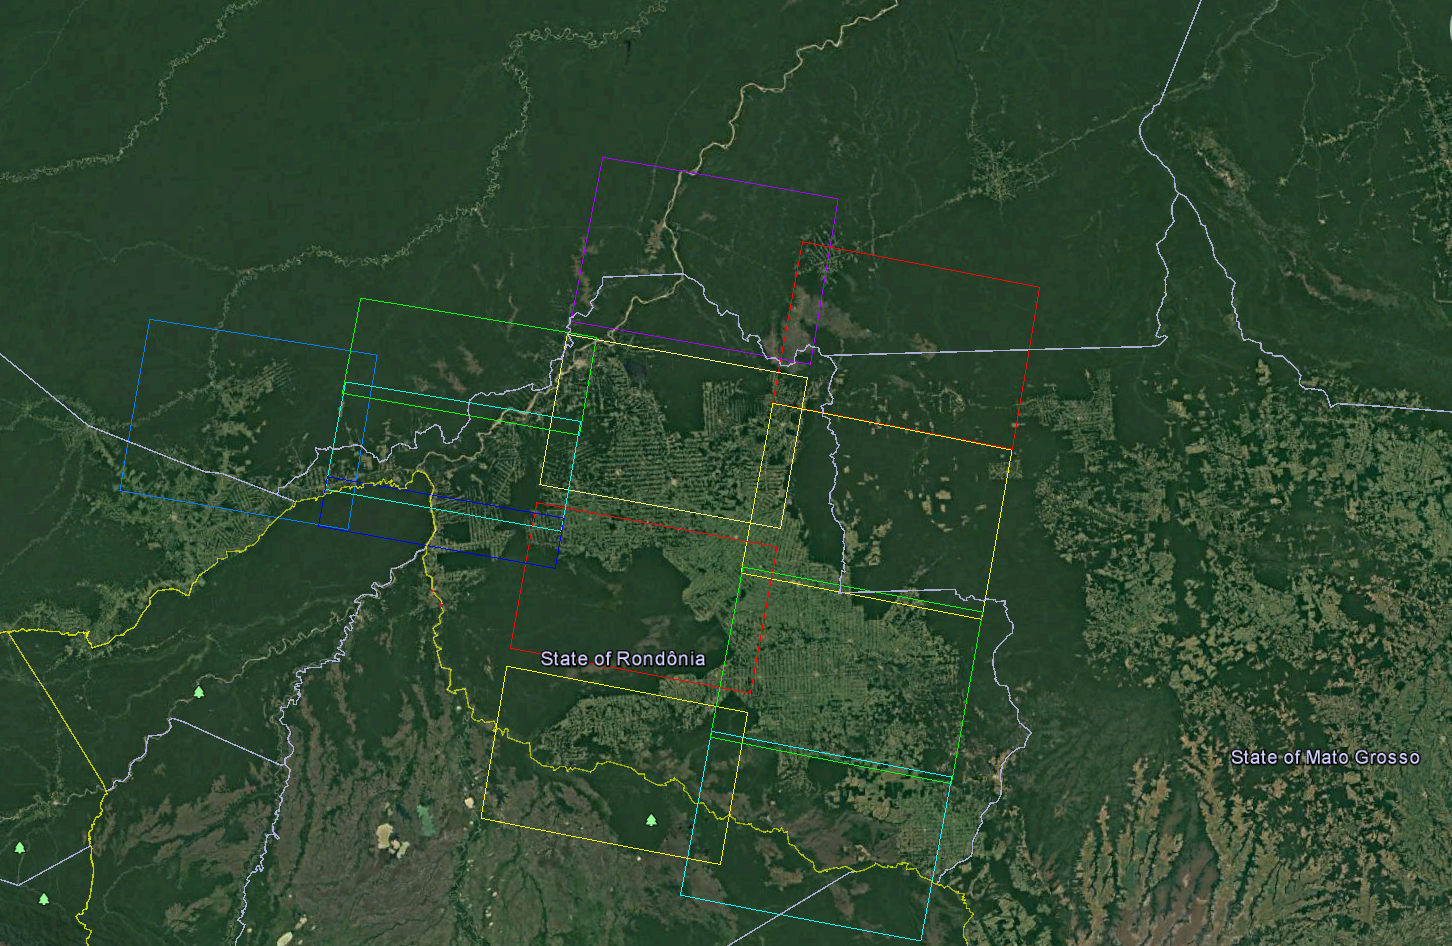
\includegraphics[width=\linewidth]{Chapter2-real/sentinel_dataset.png}
    \caption{SENTINEL-1 dataset available in Rondonia Area.}
    \label{fig:sentinel_dataset}
\end{figure}{}

SENTINEL-1 provides area coverage much greater than the TanDEM-X satellite with coverage up to 400km, but the resolution of the image is lower compared to the TanDEM-X mission. While the pixel resolution for SENTINEL-1 mission is 3.7mX14m, the TanDEM-X can provide pixels with resolution of 1.5mX1.5m. Since SENTINEL-1 provides area coverage much greater than TanDEM-X, it was chosen as main option for area monitoring in the Rondonia state as a whole. With SENTINEL-1 it was possible to cover almost the entire Rondonia state although the entire coverage was not done because there are some gaps between acquisitions as seen on \figref{fig:sentinel_dataset}. Even though the resolution for the SENTINEL-1 is much lower than the resolution of the TanDEM-X, it will be investigated on this thesis if this resolution is enough to detect new areas of deforestation. The SENTINEL-1 dataset for the Rondonia state can be seen on \figref{fig:sentinel_dataset}, where each rectangle is one acquistion made by SENTINEL-1.